\documentclass[12pt]{article}
\usepackage[a4paper]{geometry}
\usepackage[spanish,es-tabla]{babel}
\usepackage[utf8]{inputenc}
\usepackage[T1]{fontenc}
% \usepackage{fontspec}
\usepackage{graphicx}
\usepackage{times}
\usepackage{amsmath}
\usepackage{setspace}
\usepackage{enumitem}
\usepackage{fancyhdr}
\usepackage{lipsum}
\usepackage{parskip}
\usepackage[backend=biber, style=apa]{biblatex}
\addbibresource{bibliografia.bib}
\usepackage{caption}
\usepackage{floatrow}
\usepackage{titlesec}
\usepackage{titletoc}
\usepackage{appendix}
\usepackage{tabularray}
\usepackage{tocloft} 
\usepackage{titlesec}
\usepackage{physics}
\usepackage{changepage}
\usepackage[hidelinks]{hyperref} % eliminar rectangulos rojos en los links

\usepackage{titlesec}
\titleformat{\section}
  {\normalfont\fontsize{16}{16}\bfseries}{\thesection .}{0.5ex}{}
\titleformat{\subsection}
  {\normalfont\fontsize{14}{14}\bfseries}{\thesubsection .}{0.5ex}{}
\titleformat{\subsubsection}
  {\normalfont\fontsize{14}{14}\bfseries}{\thesubsubsection.}{0.5ex}{}


%-----------------CONFIGURACION-------------------------------

% Configuracion de la Pagina 
\geometry{
    a4paper,
    total={21cm,29.7cm},
    left=3cm,
    top=2.5cm,
    right=2.5cm,
    bottom=2.5cm }

\setstretch{1.5} %Interlineado a 1.5
\setlength{\parindent}{1cm} %Sangría de cada nuevo párrafo a 1cm

% Configuración del pie de página
\fancyfoot[C]{\rule{\textwidth}{0.4pt}\\ \hspace*{\fill}\fontsize{12pt}{14pt}\selectfont Título de Tesis \hspace*{\fill}\thepage} 

%\setlength{\footskip}{1.02 cm}
\setlength{\footskip}{0.5 cm}
\pagestyle{fancy} % Establecer el estilo de página como 'fancy'

\fancyhead{} % Limpiar encabezado
\renewcommand{\headrulewidth}{0pt} % Eliminar la línea de encabezado

\DefineBibliographyStrings{spanish}{ % Redefinir la cadena de texto para Bibliografía
  references = {BIBLIOGRAFÍA}, % <-- Aquí cerramos correctamente la definición}

% Configuración global de las descripciones de las figuras
\captionsetup[figure]{labelsep=period}
% Configuración global de las descripciones de las tablas
\floatsetup[table]{capposition=top}
\captionsetup[table]{labelsep=period}

% Personalización del formato del índice de figuras
\renewcommand{\cftfigpresnum}{Figura }
\renewcommand{\cftfigaftersnum}{.}
\setlength{\cftfignumwidth}{4em}

% Personalización del formato del índice de tablas
\renewcommand{\cfttabpresnum}{Tabla }
\renewcommand{\cfttabaftersnum}{.}
\setlength{\cfttabnumwidth}{4em}

% Personalizar el formato del índice general
\renewcommand{\cftsecleader}{\cftdotfill{\cftdotsep}} % Agrega puntos entre el título de la sección y el número de página
\renewcommand{\cftsecfont}{\bfseries} % Establece la fuente del título de la sección en el índice como negrita
\renewcommand{\cftsecpagefont}{\bfseries} % Establece la fuente de la página de la sección en el índice como negrita


% Definir el espaciado entre secciones y subsecciones
\titlespacing*{\subsection}{1cm}{*1.5}{*1}

% Definir el espaciado entre subsecciones y subsubsecciones
\titlespacing*{\subsubsection}{1.5cm}{*1.5}{*1}

\usepackage{fontspec}
\setromanfont[
BoldFont=Calibri Bold.TTF,
ItalicFont=Calibri Italic.ttf,
BoldItalicFont=Calibri Bold Italic.ttf,
]{Calibri Regular.ttf}

\begin{document}

%-------------------------- PORTADA -----------------
\begin{titlepage}
\centering

\includegraphics[width=13.58cm, height=3.1cm]{Logo Untref.png} 

\vspace{0.1cm}

\hspace*{-1.31cm}% Espacio horizontal de 1.31cm desde el borde izquierdo de la hoja
\begin{minipage}[t]{16cm}
\centering
\framebox[17.13cm][c]{\parbox{18.13cm}{\centering{\fontsize{16pt}{1.5pt}\selectfont INGENIERÍA EN SONIDO}}}
\vspace{0.5cm} % Espacio vertical entre el recuadro y el texto siguiente

\end{minipage}


\vspace{36pt}

{\bfseries\fontsize{22pt}{24pt} \selectfont Título de Tesis \par}

\vspace{22pt}

{\itshape\fontsize{18pt}{24pt}\selectfont \textbf{Subtítulo de la tesis (si lo tuviera)} \par}

\vspace{44pt}

{\centering\itshape\fontsize{14pt}{1pt}\selectfont Tesis final presentada para obtener el título de Ingeniero\par}
{\centering\itshape\fontsize{14pt}{1pt}\selectfont de Sonido de la Universidad Nacional de Tres de Febrero \par}
{\centering\itshape\fontsize{14pt}{1pt}\selectfont (UNTREF) \par}

\vspace{70pt}

{\bfseries\fontsize{14pt}{0pt}\selectfont TESISTA: Nombre y apellido (DNI número) \par}
{\bfseries\fontsize{14pt}{0pt}\selectfont TUTOR/A: Nombre y apellido (Ing., PhD., etc.) \par}
{\bfseries\fontsize{14pt}{0pt}\selectfont COTUTOR/A: Nombre y apellido (si lo tuviera) \par}

\vfill

\begin{table}[h]
\hrulefill \\ 
\begin{tabular}{c}
Fecha de defensa: mes y año $\lvert$ Locación (Ej. Saenz Peña), Argentina \\
\end{tabular}
\end{table}
\hrule
\end{titlepage}

\newpage
\thispagestyle{empty} % Página en blanco sin número de página, encabezado ni pie de página
\mbox{} % Contenido de la página en blanco
\newpage

%---------------------------------------------------------------
% CUERPO DEL DOCUMENTO
% Centrar título de sección

\pagenumbering{roman} % Comienza la numeración de página en números romanos
\setcounter{page}{2} % Establece el número de página según sea necesario

%-----------------Agradecimientos-----------------
\newpage 
\thispagestyle{plain} 
% \section*{AGRADECIMIENTOS} % Título centrado
\begin{centering}
\Large{\textbf{AGRADECIMIENTOS}}

\end{centering}

Se propone incluir este apartado, donde se debe agradecer primeramente a las autoridades de la Universidad, al coordinador de la carrera, al tutor y a los docentes implicados en el desarrollo de la investigación. Seguidamente agradecer a familiares o a aquellas personas que se quiera. También puede incluirse en la siguiente hoja una dedicatoria personal. A modo de ejemplo el contenido podría ser:

“En primer lugar dar gracias a la Universidad Nacional de Tres de Febrero (UNTREF), a su Rector Lic. Anibal Jozami, a todo su personal docente y no docente. Por promover un espacio ideal para el desarrollo de ideas y nuevos pensamientos y brindar a todos y cada uno de los alumnos, de esta casa de altos estudios, todos los recursos que esta institución dispone.   
Esta investigación no hubiera sido posible sin una formación académica acorde, por este motivo debo extender mi agradecimiento a los docentes de la carrera de Ingeniería de Sonido de la UNTREF, a su coordinador Ing. Alejandro Bibondo, que siendo la primera carrera de estas características del país, es muy importante contar con un cuerpo docente afín a las exigencias que este desafío propone, prestando su dedicación y vocación de enseñar. 
Un especial agradecimiento por la participación de esta tesis a la tutora Ing. Nombre Apellido, que supo transmitirme sus conocimientos y ayudarme a organizarme y fijarme un rumbo concreto y delineado, disponiendo desmedidamente de su tiempo. 
Por otra parte, quisiera hacer una mención especial al Ing. Hernan San Martin, que permitió el uso de las instalaciones de su laboratorio para poder trabajar y la disposición de todos sus recursos para que dicha investigación se realizara en tiempo y forma. 
Por último y no menos importante, quiero dar un afectuoso y cálido agradecimiento a mi familia…”

\newpage


\clearpage

\newpage
\thispagestyle{plain} % Página en blanco sin número de página, encabezado ni pie de página
\mbox{} % Contenido de la página en blanco
\newpage

%-----------------Estado del Arte-----------------
\newpage
\thispagestyle{plain} 
% \section*{DEDICATORIA} 
\textcolor{white}{
hola \\
hola \\
hola \\
hola \\
}
\begin{flushright}
\LARGE{\textbf{DEDICATORIA}}
\end{flushright}


\begin{flushright}
\textit{Elige a quién o a qué quieres dedicárselo. \\
Elegir el motivo de la dedicatoria (orientativo).}
\end{flushright}


%------------------Indices------------------------
\newpage
\renewcommand{\contentsname}{ÍNDICE DE CONTENIDOS}
\tableofcontents   % Índice General
\listoffigures  % Índice de Figuras
\listoftables   % Índice de Tablas 


%------------------Resumen------------------------

\newpage
\thispagestyle{plain} 
% \section*{\centering RESUMEN} 
\addcontentsline{toc}{section}{RESUMEN} % Agregar RESUMEN al índice
\begin{centering}
\Large{\textbf{RESUMEN}}

\end{centering}

% \raggedright
Su contenido no debe superar una página. Se indicarán los objetivos del trabajo, los métodos y resultados principales. A dos espacios debajo del resumen, en la misma página, se colocarán hasta 5 palabras clave que identifican los contenidos del trabajo.



\textbf{Palabras Clave:} 

% \end{titlepage}

%------------------Abstrac------------------------

\newpage
\thispagestyle{plain} 
% \section*{\centering ABSTRACT} 
\addcontentsline{toc}{section}{ABSTRACT} % Agregar ABSTRACT al índice
\input{secciones/0.4.abstrac}



%-----------------Introducción-----------------
\clearpage % Asegúrate de que la sección de introducción comience en una nueva página
\pagenumbering{arabic} % Restaurar numeración arábiga
\section{INTRODUCCIÓN} 
\subsection{FUNDAMENTACIÓN}

Breve fundamentación del trabajo de tesis en forma clara y concisa, estableciendo la relevancia y pertinencia del mismo en el ámbito del conocimiento donde se desarrolle. Debería establecerse la ubicación del trabajo dentro del estado del arte, pero sin desarrollar el detalle que se hará en los siguientes capítulos. No deben incluirse resultados ni detalles experimentales. Es deseable que no supere las 4 hojas.

\subsection{OBJETIVOS}

\subsubsection{Objetivo general}

Resumir en una sola frase el objetivo de la investigación.

\subsubsection{Objetivo especifico}

\begin{itemize}
    \item Listar los distintos objetivos siguiendo un orden metodológico. Recordar que la revisión bibliográfica no es un objetivo específico
    \item Identificar los recintos, paramentos verticales y horizontales y revestimientos fonoabsorbentes que conforman el estudio de grabación.
    \item Realizar simulaciones de tiempo de reverberación e indicadores de inteligibilidad de la palabra mediante el programa EASE.
    \item Obtener el índice de reducción sonora R de los distintos detalles constructivos mediante el programa de predicción INSUL.
    \item 	Realizar mediciones in situ de los descriptores de acondicionamiento acústico según norma ISO 3382-1.
    \item	Realizar mediciones in situ según norma ISO 16283-1 para obtener los índices de aislamiento acústico a ruido aéreo.
    \item Comparar los resultados de las simulaciones respecto a los valores obtenidos de las mediciones.
    \item Realizar propuestas de mejora a implementar.
\end{itemize}

\subsection{ESTRUCTURA DE LA INVESTIGACIÓN}

Indicar en distintos párrafos el contenido de cada uno de los capítulos que conformarán la tesis.

En el capítulo 2 se presenta el marco teórico donde se detallan los parámetros e indicadores necesarios para el desarrollo de la investigación.


En el capítulo 3 se hace referencia a aquellas investigaciones vinculadas con el tema a desarrollar en esta tesis.


En el capítulo 4…



\clearpage



%-----------------Marco Teorico-----------------
\newpage
\section{MARCO TEÓRICO} 
    En el Marco Teórico debemos incorporar la bibliografía, artículos de revistas, ponencias de congresos, links de Internet o todo aquello que haya contribuido a formar el cuerpo del saber sobre el que va a basarse la investigación, incorporando los procesos y ecuaciones necesarios.

Puede ser uno varios capítulos donde se detallen los parámetros, indicadores y conceptos teóricos referentes al tema a tratar. Se recomienda no utilizar conceptos muy básicos, como definición de nivel de presión sonora, ponderación A, etc.


%-----------------Estado del Arte-----------------
\newpage
\section{ESTADO DEL ARTE} 
    Puede ser uno o varios capítulos que desarrollen el estado del arte del área de conocimiento donde se inserta la tesis. La profundidad del enfoque en el tratamiento de los temas debe ser adecuado para el entendimiento posterior de los resultados y discusiones de la tesis. No es necesario que sea autocontenido, es recomendable el uso amplio de referencias a trabajos previos que se encuentren en la literatura abierta sobre el tema.

%-----------------Diseño de la investigacion-----------------
\newpage
\section{DISEÑO DE LA INVESTIGACIÓN} 
    \input{secciones/4.diseño_de_la_investigacion.tex}

%-----------------Validacion de las pruebas-----------------
\newpage
\section{VALIDACIÓN DE LAS PRUEBAS} 
    Las pruebas se validarán siguiendo los criterios estadísticos que permiten determinar la existencia o no de errores en alguna o algunas encuestas y considerar si son incluidas o no en el conjunto de respuestas. Como las pruebas no se realizarán todavía, deben plantearse los métodos elegidos y explicarlos.

%-----------------Analisis de los resultados-----------------
\newpage
\section{ANÁLISIS DE LOS RESULTADOS: APLICACIONES ESTADÍSTICAS} 
    Aquí se aplicarán los métodos estadísticos que nos permitan concluir los resultados y proyectar diferentes facetas de los datos obtenidos. Como las pruebas no se realizarán todavía, deben plantearse los métodos elegidos y explicarlos.

%-----------------Conclusiones-----------------
\newpage
\section{CONCLUSIONES} 
    En las conclusiones del Plan de Investigación, debe plantearse cómo será la exposición de los resultados y qué es lo que se espera obtener en resumen de las pruebas que se realicen.

%-----------------Linea futuras de Invetigacion-----------------
\newpage
\section{LÍNEAS FUTURAS DE INVESTIGACIÓN} 
    Las líneas futuras de investigación dentro del plan, suponen expresar qué posibles cuestiones que se encontrarán se dejarán para ser profundizadas más adelante por otras investigaciones.
\textcolor{white}{
\parencite{Beranek2005ConcertHA} 
\parencite{busch2005noise}
\parencite{Call2007SoundP}
\parencite{Gardner2002}
\parencite{iso1996-2}
\parencite{kracht2007noise}
\parencite{Lawson2010SoundIntensity}
\parencite{MacLeod2007QuietingWeinberg}
\parencite{Mazer2012Creating}
\parencite{Orellana2006NoiseIT}
\parencite{richardson2009development}
\parencite{Ryherd2008CharacterizingNA}
\parencite{sanz2012tecnicas}
\parencite{Taylor1958NoiseCI}
\parencite{Tsiou2008Noise}
\parencite{text-to-speech-ibm}
\parencite{West2008NoiseIH}}

%-----------------Bibliografia-----------------
\newpage

\printbibliography[title={Bibliografia}]

%-----------------ANEXO-----------------
\newpage
\appendix
\section*{ANEXO I. \quad FORMATO INTERNO} 
    \subsection*{AI 1. \textit{Numeración}}

Las páginas serán enumeradas a partir del Índice de Contenidos, con números romanos colocados en la parte media inferior de cada página. A partir de la Introducción, todas las páginas serán enumeradas con números arábigos ubicados en la parte inferior derecha. No usar la palabra “página” antes de la numeración de las páginas.

\subsection*{AI 2. \textit{Palabras Clave (tamaño 10)}}

Debajo del resumen deberán indicarse hasta cinco (5) palabras clave, también conocidas como descriptores. En la sección del resumen en inglés (abstract) deberán también incluirse las palabras clave (keywords). Se colocarán inmediatamente debajo del resumen (abstract) con la indicación en negrita Palabras Clave (Keywords) y a continuación en la misma línea las palabras. 

\subsection*{AI 3. \textit{Títulos y Subtítulos}}

El título de los capítulos debe numerarse con número arábigo consecutivos, y ser escrito con letra mayúscula y en negrita en tamaño 16 puntos escritos a partir del margen izquierdo en una nueva página. El subtítulo (o si corresponde, el inicio de un texto), comenzará 1 espacio más abajo. El subtítulo será precedido por un número arábigo y se escribirá con letra mayúscula en negrita y tamaño 14 puntos, escrito a partir del margen izquierdo. El subtítulo del 3er. orden (o si corresponde un texto), comenzará 1 espacio más abajo. Los subtítulos de 3er. orden podrán ser idénticos al anterior, pero escritos con letra minúscula (la primera con mayúscula), sin negritas, y el texto comenzará una línea más abajo. Si a continuación del subtítulo de 3er. orden se escribe un subtítulo de 4º orden deberá dejarse un espacio. Los subtítulos de 4º, 5º u orden superior, serán idénticos al de 3er orden y el texto comenzará en la misma línea.

Las palabras y/o frases no deben ser abreviadas en títulos y resumen la primera vez que aparecen. 

\subsection*{AI 4. \textit{Figuras, Tablas, Ecuaciones y Notas al pie (tamaño 10)}}

Las Figuras, Ilustraciones (Estilo Figura) y Tablas deben ser colocadas en secuencia en el texto, y siempre que sea posible próximas de donde son indicadas. Las figuras deben ser de buena calidad (en una impresión deberían notarse todos los detalles que fueran importantes) y llevar una leyenda concisa en su parte inferior. Todas las ilustraciones y figuras deben ser numeradas (Ej “Figura \ref{fig:Tiempo de reverberacion}” etc.) nunca excediendo los márgenes de impresión. En caso de incorporarse a la sección de anexo, la numeración debe estar antepuesta por la letra A y reestablecer la misma a 1 (ej ''Figura \ref{fig:Comparativa R}”).

Las letras en los dibujos o gráficos no deberían ser menores a 1,5 mm de alto. Si es posible, las letras en todas las ilustraciones deben ser del mismo tamaño, y usar el idioma castellano (no inglés). Se recomienda no utilizar solamente colores para identificar características de un gráfico (en caso de mediciones, utilizar símbolos diferentes con cada color, así además se pueden identificar por la forma). Las leyendas de las Tablas (Ej “Tabla 1”) deben ser posicionadas centradas encima de las mismas (Estilo Título Figuras). Tanto para las Figuras como para las Tablas, junto a la identificación debe suministrarse una pequeña descripción explicativa del contenido. En caso de incorporarse a la sección de anexo, la numeración debe estar antepuesta por la letra A y reestablecer la misma a 1 (ej “Tabla \ref{Tab:1}”).

Si la Figura o Tabla es una copia sacada de una de las fuentes bibliográficas, es preferible vectorizar mediante algún programa de dibujo para mejorar la resolución. También debe constar en el título la fuente mediante el número de referencia bibliográfica.
Las ecuaciones y expresiones matemáticas deben estar centradas y numeradas en secuencia, con el número de la ecuación justificado a la derecha y entre paréntesis, utilizando numeración arábiga.
En caso de utilizar notas al pie deben estar referidas con algún símbolo en superíndice (Ej texto†) en el cuerpo del texto y en el pie de la misma página referir el comentario en letra tamaño 10 interlineado simple. Se sugiere que la nota al pie no supere los tres renglones.

Las ecuaciones y expresiones matemáticas deben estar centradas y numeradas en secuencia, con el número de la ecuación a la derecha y entre paréntesis, utilizando numeración arábiga. En ecuaciones de varias líneas, la numeración debe ser ubicada en la última línea. Las fórmulas y el texto deben ser separados por una línea. Las ecuaciones deben ser hechas en la misma fuente del texto, con los índices 3 puntos abajo. Deben usarse símbolos convencionales y unidades SI. Las ecuaciones deben ser citadas en el texto (''Ecuación \eqref{eq: LF}", etc.).

En el texto debe definirse cada símbolo, con sus unidades, y representadas en formato itálica (''donde S es la superficie del elemento en $m^2$, TR es el tiempo de reverberación del recinto a una cierta frecuencia expresado en segundos y $\alpha$ es el coeficiente de absorción sonora, adimensional”).

\begin{equation}
    \label{eq: LF}
    \tau_{d} = \frac{\int_{0}^{\theta_{lim}} \tau \sin \sin \theta \cos \cos \theta \ \dd \theta}{\int_{0}^{\theta_{lim}} \sin \sin \theta \cos \cos \theta \ \dd \theta}
\end{equation}

Para ingresar ecuaciones y se enumeren automáticamente, pueden usar el formato de la ecuación anterior (es una tabla de 1 fila y dos columnas, la primera celda está el editor de ecuaciones y en la segunda celda el número de ecuación): 


    \begin{figure}[h]
        \centering
        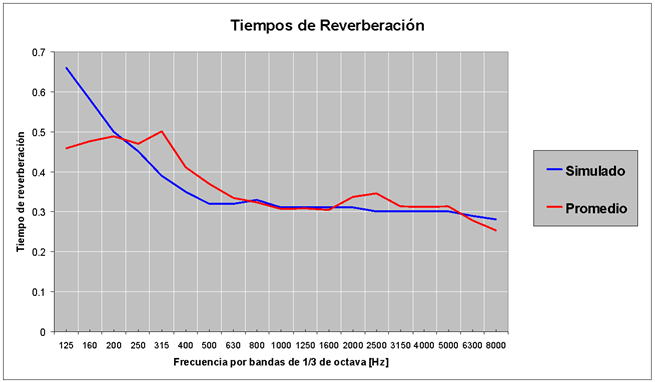
\includegraphics[scale=0.9]{figuras/Tiempo de Reverberacion.png}
        \caption{Comparación de los tiempos de reverberación entre el promedio espacial y la simulación del Hall 4.}
        \label{fig:Tiempo de reverberacion}
    \end{figure}

    \begin{figure}[h]
        \centering
        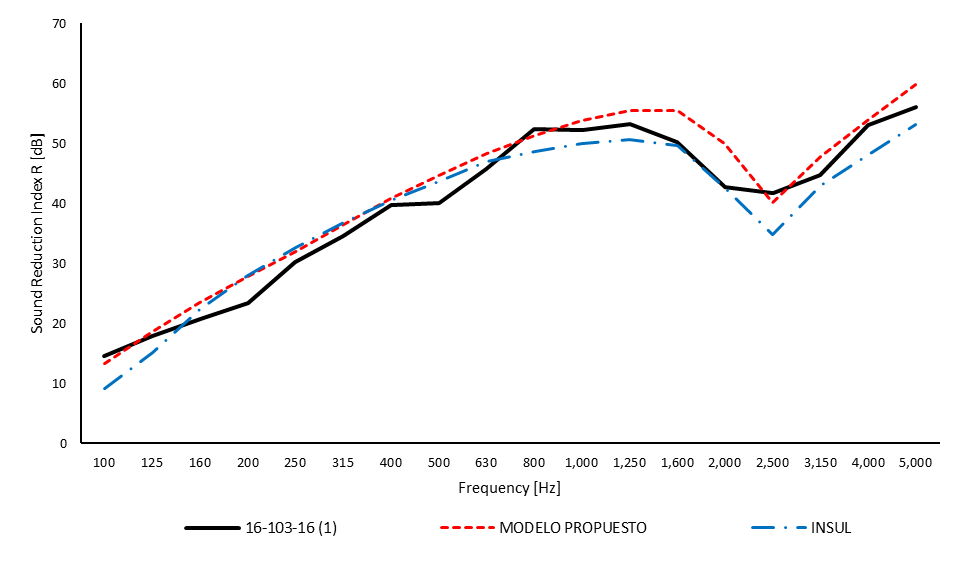
\includegraphics[scale=0.9]{figuras/Comparacion reduccion sonora R.png}
        \caption{Comparativa de los índices de reducción sonora R entre la medición de laboratorio, la predicción del modelo propuesto y el programa INSUL para el caso 1.}
        \label{fig:Comparativa R}
    \end{figure}


\begin{table}
\centering
\begin{tblr}{
  cells = {c},
  hline{1-2,7} = {-}{},
}
\textbf{Material}  & \textbf{Espesor \\\ [mm]} & {\textbf{Densidad}\\\textbf{$[Kg/m^3]$}} & {\textbf{Young}\\\textbf{[GPa]}} & \textbf{Poisson} & {\textbf{Factor de perdidas}\\\textbf{interno}} \\
hormigon  & 50,8; 101,6; 140; 160(x2);& 2100 & 30 & 0,2 & 0,03 \\
Vidrio    & 180; 200; 220; 240              & 2500 & 71 & 0,23& 0,02  \\
placa de yeso & 6,4; 9,5; 12,7; 15.9   & 768  & 2 &  0,23& 0,01  \\
laminado  &  3.2; 6.4                       & 1250 & 3 &  0,15& 0,03  \\
HDF       &  50; 70(x4); 100                &  900 &  3.5& 0,2& 0.005
                                       
\end{tblr}
\caption{Lista de materiales utilizados en la comparativa y sus características físicas.}
\label{Tab:1}
\end{table}

\subsection*{AI 5. \textit{Bibliografía}}
Las referencias a la bibliografía utilizada deberán registrarse en el texto entre corchetes con un número arábigo (Ej [5]). La numeración debe ser consecutiva. En caso de citarse más de una referencia se hará separadas por comas dentro del corchete (Ej [5, 18]) y en caso de necesitar la cita de una sucesión consecutiva de referencias se escribirán separadas por una línea (Ej [5-11]).

La numeración correspondiente a las referencias se podrá incluir al final de la tesis (como se especifica más arriba en la descripción de la Estructura) o bien al final de cada capítulo incluyendo solamente las referencias de ese capítulo. Al utilizar las referencias por capítulo pueden quedar referencias repetidas entre capítulos; en este caso cada capítulo debe ser autocontenido con respecto a las referencias.

\end{document}


